\documentclass[journal,twoside,web]{ieeecolor}
\usepackage{generic}
\usepackage{cite}
\usepackage{amsmath,amssymb,amsfonts,listings}
\usepackage{algorithmic}
\usepackage[justification=centering]{caption}
\usepackage{float}
\usepackage[dvipsnames]{xcolor}
\usepackage{graphicx}
\usepackage{textcomp}
\usepackage[UTF8]{ctex}
\usepackage[colorlinks, linkcolor=blue, urlcolor=red]{hyperref}
\setCJKfamilyfont{myfont}{msyhbd.ttc}
\newcommand{\SetFont}{\CJKfamily{myfont}}
%\SetFont{生僻字}
\def\BibTeX{{\rm B\kern-.05em{\sc i\kern-.025em b}\kern-.08em
    T\kern-.1667em\lower.7ex\hbox{E}\kern-.125emX}}
\markboth{智能工程学院  智能科学与技术}
{无人系统导论作业}
\lstset{
    language=Python,
    basicstyle=\ttfamily\small,
    keywordstyle=\bfseries\color{NavyBlue},
    commentstyle=\itshape\color{red!50!green!50!blue!50},
    stringstyle=\bfseries\color{PineGreen!90!black},
    emph={self}, 
    emphstyle=\bfseries\color{Rhodamine},
    backgroundcolor=\color{black!3},
    frame=shadowbox,
    frameround=fttt,
    numbers=left,
    numberstyle=\tiny,
    stepnumber=1,
    numbersep=5pt,
    breaklines=true,
    columns=flexible,
    xleftmargin=2em,
    xrightmargin=0em,
    aboveskip=1em,
    framexleftmargin=2em,
    escapeinside=``,
}

\begin{document}
\title{基于ROS的多机器人导航与编队仿真实现}
\author{陈海弘,方唯特,蒋奥周,刘仲晗
\thanks{陈海弘,23354049,(e-mail: chenhh93@mail2.sysu.edu.cn),}
\thanks{方唯特,23354057,(e-mail: fangwt5@mail2.sysu.edu.cn),}
\thanks{蒋奥周,23354081,(e-mail: jiangaozh@mail2.sysu.edu.cn),}
\thanks{刘仲晗,23354117,(e-mail: liuzhh268@mail2.sysu.edu.cn)。}
}

\maketitle

\begin{abstract}
本实验基于 ROS 1 (Noetic) 开展多机器人导航与编队仿真,利用 Gazebo 和 RViz 实现导航、避障和队形维持等功能,探索多机器人系统的协同能力。实验展示了领航者-跟随者策略的应用,并分析了方法的优点和局限。通过实验验证了多机器人编队在智能交通、灾害救援、农业自动化等场景中的潜力,为无人系统的实际应用提供了技术支撑。%这是摘要
\end{abstract}

\begin{IEEEkeywords}
ROS, 多机器人系统, Gazebo, RViz, 导航与编队, 领航者-跟随者, 仿真, 无人系统%这是关键词
\end{IEEEkeywords}
\section{实验背景与意义}
本实验旨在基于 ROS 1 (Noetic) 探索多机器人导航与编队仿真的实现,
通过开源资源和相关教程深入了解 ROS 在多机器人系统中的应用潜力。
核心目标是在仿真环境中测试机器人导航与编队功能,探索传感器数据可视化及协同工作机制,
这些技术在实际生活中具有广泛的应用价值。

近年来,无人系统技术飞速发展,无人机、无人车及无人船等在军事、工业及科研领域的应用逐渐成熟。
多无人系统的协作能力成为完成复杂任务的关键,例如在灾害救援中协作搜索与物资投放,
在军事领域执行目标侦察和区域监控等任务。

\subsection*{多无人系统的核心功能}
导航与编队 是多无人系统协作的核心内容。通过自主导航,无人系统能够避障并到达目标;
协同编队则可保持队形并完成复杂任务。这种协作能力对提升任务效率及操作安全性至关重要,
为军事智能靶场、环境监测、物流运输、搜救任务等应用场景提供了强有力的支持。

\subsection*{多领域的应用场景}
	1.	智慧城市与智能交通:
多机器人系统可用于环境监控、城市巡逻及智能交通管理,例如夜间清洁机器人或24小时智能巡逻机器人。
同时,自动驾驶与无人机配送服务依赖复杂导航算法与高效协同机制,确保安全可靠。
	
2.	灾害响应与救援:
多机器人系统在地震、洪水等灾害中执行搜救任务,利用传感器收集现场信息并协助制定救援计划。
它们也可替代人类进入高风险区域执行探测或运输任务,降低风险。
	
3.	农业自动化:
智能农业利用多机器人系统精准完成播种、施肥、采摘等工作,提升效率、减少环境影响。
无人机与地面机器人结合实现作物健康监测,快速发现病虫害并采取措施。
	
4.	医疗保健:
医院中,移动机器人承担药品配送与患者引导等任务;
远程医疗机器人平台使医生能远程操作设备,在偏远地区或紧急场景中实施医疗援助。
	
5.	军事应用:
	
•	侦察与监视:部署无人飞行器与地面车辆获取实时情报。
	
•	作战支援:用于物资运输、伤员撤离及火力掩护。
	
•	排爆与拆弹:特种机器人精确拆除爆炸物,保障安全。
	
•	训练模拟:通过仿真环境提升战术训练效率,降低成本。
	
•	边境巡逻:自主巡逻机器人全天候执行监控任务,提升边防效率。

\subsection*{仿真工具的重要性}
本实验采用 Gazebo 和 RViz 两款工具,结合 ROS 进行仿真开发:


•	Gazebo 提供逼真的3D物理仿真环境,支持碰撞检测、摩擦力及多传感器模型,可用于测试机器人算法与多机器人协作。

•	RViz 提供直观的数据可视化界面,用于展示传感器数据、机器人状态及路径规划结果,帮助研究人员快速诊断问题并优化性能。

通过 Gazebo 和 RViz 的支持,研究人员能够在无硬件条件限制下高效开发、测试和调试算法。
这不仅加速了多无人系统的技术进步,也为其在空地联合、海空协作等领域的拓展奠定了基础。

综上所述,本实验在仿真中探讨多机器人系统的导航与协作潜力,
不仅为科技进步提供方向,更能为实际应用场景带来创新解决方案。
\section{导航与编队功能}
多移动机器人编队主要需要解决两个关键问题:一是编队队形的形成,二是在动态环境中维持该队形。
队形形成是指在复杂环境中,多个机器人初始时随机分布,通过自身的传感器信息及与其它机器人之间的通信和协作,
自组织成一个适合执行特定任务的稳定队形。一旦队形建立,接下来的关键挑战是确保这个队形能够在运动过程中保持不变,
即使面对环境变化或外部干扰。

本次实验采用了基于领航者-跟随者(Leader-follower)的编队策略,这是一种广泛应用的方法,
其核心思想是将编队中的成员明确区分为两类角色:


领航者(Leader):负责接收并执行全局路径规划指令,引领整个编队的方向和速度。

跟随者(Follower):根据自身与领航者之间的相对位置关系,
调整自己的姿态和速度,以维持预设的队形结构,并进行必要的避障操作。

方法优势

1. 简化控制系统:领航者-跟随者的架构使得编队控制逻辑更加直观和易于实现。编队中只需对领航者设定期望路径,减少了整体系统的复杂性。

2. 灵活性高:能够快速响应新的任务需求,例如改变领航者的路径规划即可调整编队的整体方向。

3. 易于扩展:随着编队规模扩大,只需增加跟随者数量而不需要显著改动现有控制策略,具有良好的可扩展性。

方法局限


1. 高度依赖领航者:编队的成功运作很大程度上取决于领航者的可靠性和性能。
如果领航者出现故障或失去联系,可能会导致整个编队失控。因此,领航者的冗余设计和容错机制至关重要。

2. 响应延迟:由于跟随者依赖于领航者的状态更新来进行自我调整,当编队较大时,这种依赖可能导致响应延迟,影响队形的即时性和稳定性。

3. 通信要求较高:为了保证跟随者能及时准确地获取领航者的最新状态信息,编队内部需要维持有效的通信链路,这在复杂或动态环境中可能构成挑战。
 
\section{仿真平台与实现}
我们在配置ROS环境的时候遇到了一些问题,ROS编译过程中出现找不到Config.cmake包之类的输出。
比如缺少gazebo\_rosConfig.cmake,gazebo\_ros-Config.cmake,camera\_info\_managerConfig.cmake。

通过运行以下代码,安装了缺失的文件:
\begin{lstlisting}
    sudo apt-get install ros-melodic-gazebo-ros
\end{lstlisting}
之后的包缺失也是通过这样的方法解决的。

通过终端进入ROS工作空间,编译项目,并且启动仿真环境Gazebo。
\begin{lstlisting}
cd catkin\_ws
source devel/setup.bash
catkin\_make
roslaunch ares\_gazebo ares\_cloister\_gazebo.launch
\end{lstlisting}

\begin{figure}[H]
    \centering
    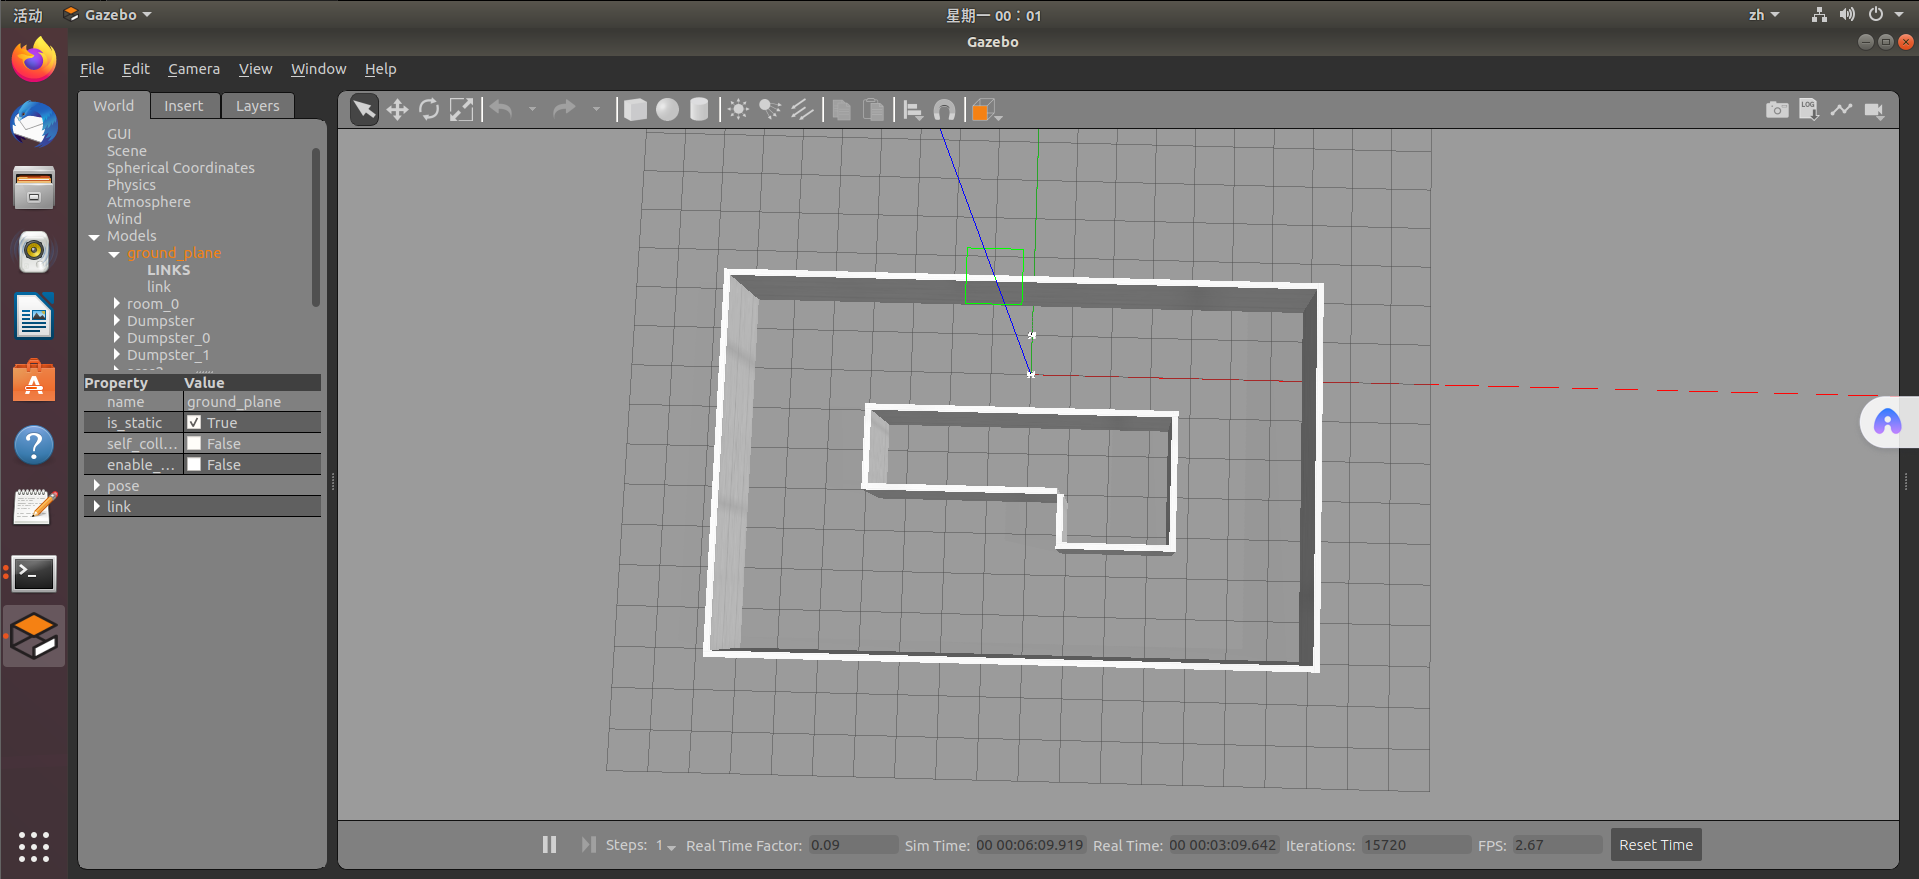
\includegraphics[width=0.8\linewidth]{img/1.jpg}
    \caption{Gazebo仿真环境}
\end{figure}

打开rviz,进行领航者导航:
\begin{lstlisting}
roslaunch ares\_navigation navigation\_demo.launch
\end{lstlisting}

\begin{figure}[H]
    \centering
    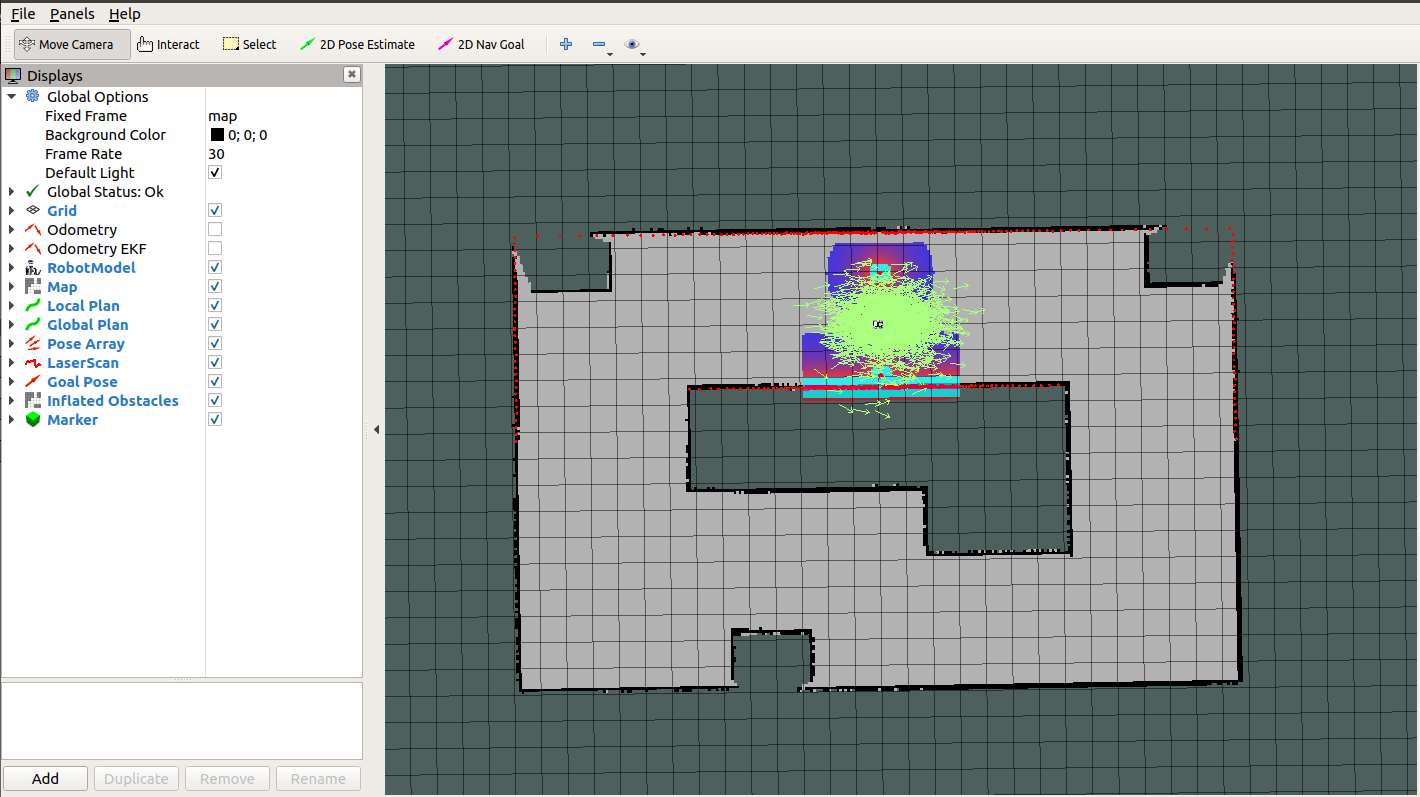
\includegraphics[width=0.8\linewidth]{img/2.jpg}
    \caption{RViz导航界面}
\end{figure}

启动编队程序:
\begin{lstlisting}
roslaunch stage\_first OnYourMarkGetSetGo.launch
\end{lstlisting}

\begin{figure}[H]
    \centering
    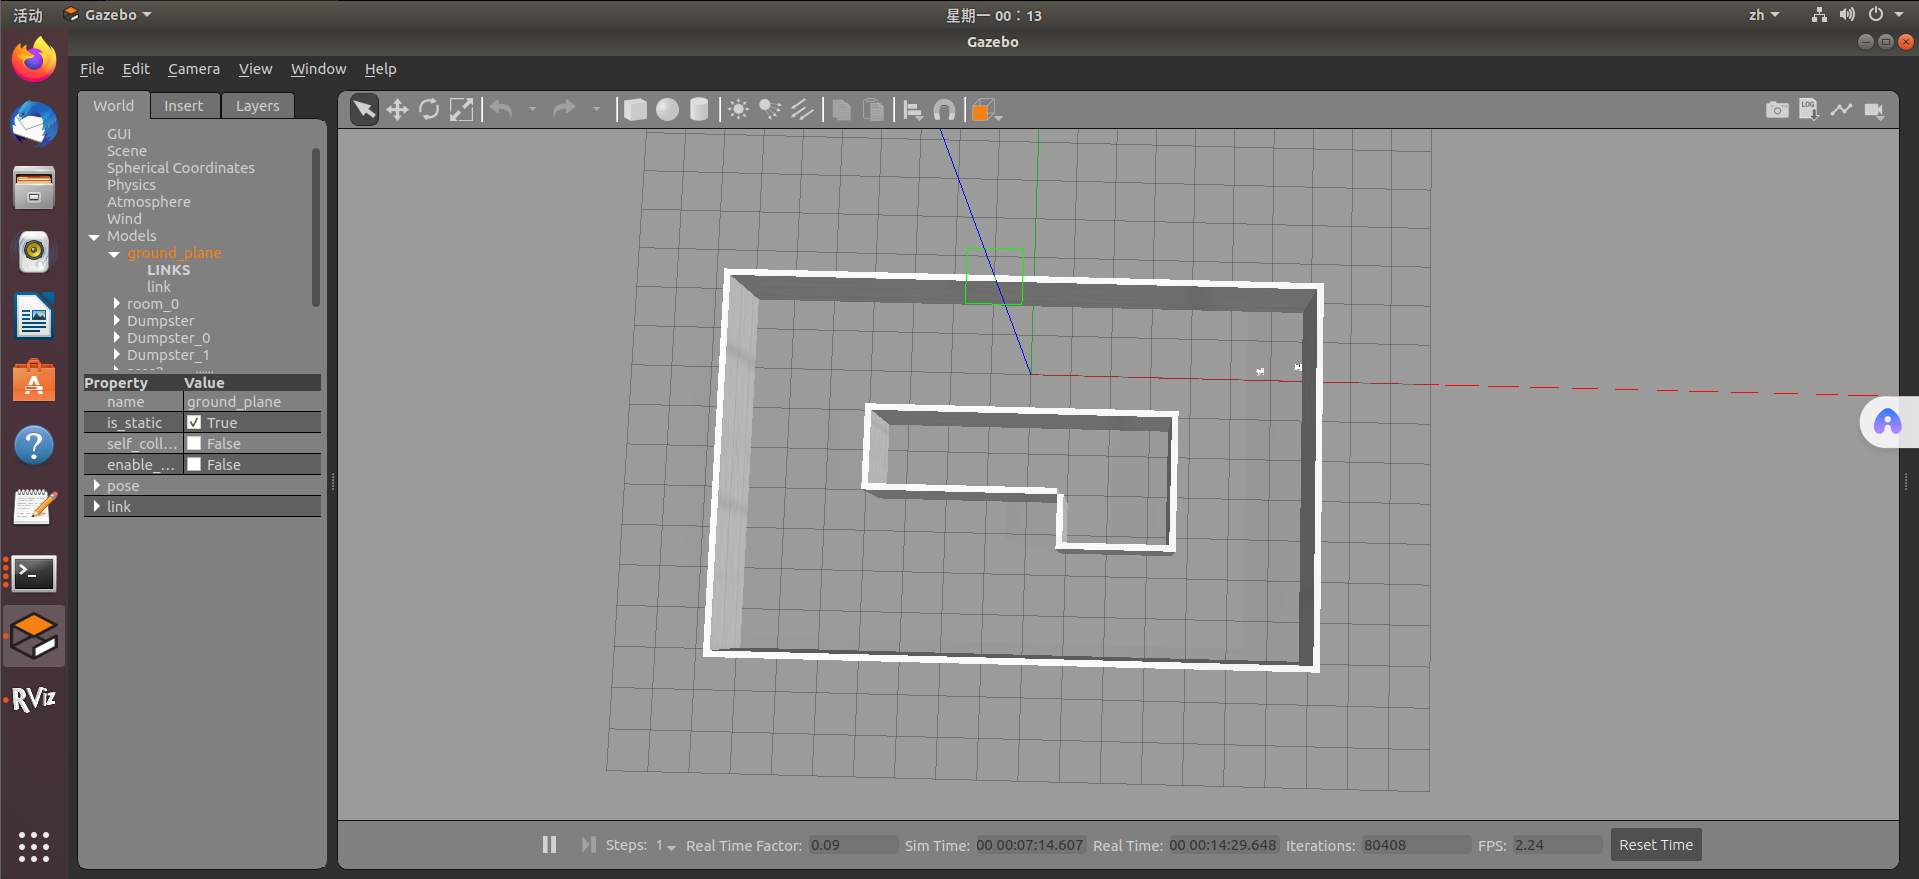
\includegraphics[width=0.8\linewidth]{img/3.jpg}
    \caption{编队仿真效果}
\end{figure}

\section{实验结果与分析}
 
在本部分实验中,我们利用ROS(Robot Operating System)和Gazebo仿真软件,在Ubuntu 18.04系统上进行了多机器人系统的跟随和编队仿真。实验的准备工作包括安装ROS Noetic版本和Gazebo,创建ROS工作空间,并下载实现跟随和编队功能的ROS包。
 
\subsection*{实验准备}
\subsubsection*{环境搭建}
\begin{itemize}
   \item 安装ROS Noetic:根据官方文档,通过apt-get命令安装了ROS Noetic及其依赖项。
   \item 安装Gazebo:选择了与ROS Noetic兼容的Gazebo版本进行安装。
   \item 创建ROS工作空间:使用catkin工具创建了一个新的ROS工作空间,用于存放所有相关的包和配置文件。
   \item 下载ROS包:从GitHub或其他开源平台下载了实现跟随和编队功能的ROS包,并将其添加到ROS工作空间中。
\end{itemize}
 
\subsection*{实验步骤}
\subsubsection*{启动仿真环境}
\begin{enumerate}
   \item 设置工作目录为ROS工作空间,确保所有必要的脚本和配置文件都在正确的路径下。
   \item 使用roslaunch命令启动Gazebo仿真环境。这一步骤加载了预设的仿真场景,并初始化了所有必要的节点和服务。
   \item 在Gazebo中加载机器人模型,并配置它们的物理属性和传感器,如激光雷达、摄像头等,以便它们能够在仿真环境中进行导航。
\end{enumerate}
 
\subsubsection*{导入和测试跟随算法}
\begin{enumerate}
   \item 导入跟随算法:该算法允许机器人根据领头机器人的位置和速度进行调整,保持一定的距离和方向。
   \item 测试跟随功能:在Gazebo中启动跟随算法后,观察到机器人能够正确跟随领头机器人。通过调整控制参数,如跟随距离和速度,优化了跟随性能。
\end{enumerate}
 
\subsubsection*{导入和测试编队算法}
\begin{enumerate}
   \item 导入编队算法:使机器人能够根据预设的编队形状进行移动,保持相对位置不变。
   \item 测试编队功能:在Gazebo中启动编队算法后,注意到机器人能够形成稳定的编队并移动。通过调整编队间距和其他参数,提高了编队的一致性和稳定性。
\end{enumerate}
 
\subsubsection*{监控和调整}
\begin{itemize}
   \item 使用RViz监控机器人的状态,包括位置、速度和传感器数据。RViz提供了直观的图形化界面,方便实时查看机器人的行为。
   \item 根据仿真结果,对机器人的控制参数进行了调整,如跟随距离和编队间距,并对跟随和编队算法进行了优化,以提高机器人的响应速度和稳定性。
\end{itemize}
 
\subsection*{数据分析}
\begin{itemize}
   \item 记录关键数据:如机器人的位置轨迹和编队形状的变化,并对这些数据进行了详细的分析。
   \item 评估算法性能:通过对比不同参数设置下的仿真结果,评估了跟随和编队算法的有效性,并发现了潜在的改进点。
\end{itemize}
 
\subsection*{实验结束}
\begin{itemize}
   \item 关闭仿真环境,确保所有进程正常终止。
   \item 保存代码和配置文件,便于后续分析和改进。
\end{itemize}
 
\subsection*{技术细节展示}
\begin{itemize}
   \item \textbf{初始布局}:展示了机器人在仿真开始时的初始位置和配置。
   \item \textbf{路径规划}:说明了机器人如何根据内置的路径规划和避障算法动态调整路径,以避免碰撞并继续向目标点移动。
   \item \textbf{跟随和编队}:展示了机器人根据算法调整它们的位置以实现跟随和编队的过程。
\end{itemize}
 
通过这两幅图,我们可以清晰地观察到机器人在仿真环境中的交互和协同工作。例如,在第二幅图中,至少有一个机器人已经开始沿着路径移动,而其他机器人则保持在起始位置。这种可视化有助于评估多机器人系统的性能,并为进一步的研究提供直观的参考。
 
\subsection*{总结}
 
综上所述,本实验不仅达成了既定目标,还揭示了ROS系统在多机器人导航与编队仿真方面的巨大潜力。通过这次实践,我们掌握了关键技术的应用方法,并积累了丰富的开发和调试经验。实验表明,合理的环境预设、模块化设计以及详细的实验记录对于成功实现复杂的多机器人系统至关重要。
 
此外,我们认识到硬件验证和可视化工具的重要性。将仿真结果应用于真实机器人平台可以验证算法的实际性能,而增强的可视化工具则有助于更直观地理解和优化系统行为。未来的研究可以在这些基础上进一步探索,例如引入更多类型的传感器、扩大应用场景范围,以及开发更加智能的路径规划和编队控制算法。
 
总之,本实验不仅巩固了现有的理论知识,还为未来的机器人研究提供了宝贵的经验和参考方向。无论是改善民生福祉还是加强国防建设,多机器人系统都展现出了巨大的潜力和发展前景。
 

\section*{无人系统自主导航仿真实验}
 
在利用ROS(Robot Operating System)和Gazebo进行的无人系统自主导航仿真实验中,我们构建了一个复杂而逼真的环境,模拟了机器人需要导航的真实场景。以下是对整个实验过程的详细描述。
 
\subsection*{仿真环境构建}
\subsubsection*{路径设计}
我们在Gazebo仿真窗口中构建了一个由白色线条构成的复杂路径,这些线条代表了机器人需要导航的路线。此路径包括直线段、曲线段以及多个转弯点,旨在模拟真实的道路环境,增加了实验的挑战性。
 
\subsubsection*{机器人模型放置}
在路径的起点,我们放置了一个黑色的矩形机器人模型,这标志着机器人的初始位置。该机器人模型配备了激光雷达传感器和其他必要的传感器,如IMU(惯性测量单元)和摄像头,以便全面感知周围环境。
 
\subsection*{实时监控与数据可视化}
\subsubsection*{RViz显示窗口}
通过RViz的显示窗口,我们实时监控了机器人的传感器数据和导航信息:
\begin{itemize}
   \item \textbf{绿色点云}:由机器人携带的激光雷达传感器实时扫描周围环境并构建的地图。点云数据直观地展示了机器人视野内的障碍物分布。
   \item \textbf{紫色箭头线}:代表了机器人的导航路径或目标方向。这条线根据路径规划算法动态更新,反映了机器人当前的目标和移动方向。
\end{itemize}
 
\subsection*{导航过程}
随着仿真的进行,机器人模型从起点出发,沿着规划的路径移动。在RViz中,我们观察到机器人的实时位置和导航状态的更新:
\begin{itemize}
   \item 绿色的点云随着机器人的移动而更新,显示了机器人周围环境的动态变化。
   \item 紫色的箭头线也相应调整,以反映机器人在避开障碍物后的新路径。
\end{itemize}
 
\subsection*{日志信息监控}
在实验过程中,我们还密切监控了终端窗口中的日志信息。这些信息记录了机器人导航过程中的关键事件,如“Get new plan”(获取新计划)和“Goal reached”(到达目标)。这些日志信息为我们提供了宝贵的反馈,帮助我们了解机器人的导航状态和任何可能发生的问题。例如:
\begin{itemize}
   \item “Get new plan”表示机器人正在重新计算路径,通常是因为遇到了新的障碍物或环境变化。
   \item “Goal reached”表示机器人已经成功到达预定的目标点。
\end{itemize}
 
\subsection*{导航算法开发与调整}
在整个实验过程中,我们通过编写和调整导航算法,使机器人能够根据激光雷达传感器提供的数据,实时构建环境地图并规划路径。具体步骤包括:
\begin{enumerate}
   \item \textbf{环境建模}:使用SLAM(同步定位与地图构建)算法,机器人可以逐步构建其所在环境的地图。
   \item \textbf{路径规划}:采用A*或RRT*等路径规划算法,为机器人生成最优路径。
   \item \textbf{避障控制}:当机器人检测到前方有障碍物时,避障算法会自动调整路径,确保机器人安全绕过障碍物并继续向目标前进。
\end{enumerate}
 
\subsection*{实验结果分析}
通过RViz和终端日志,我们实时监控并调整机器人的导航行为,确保了自主导航任务的顺利完成。实验结果表明:
\begin{itemize}
   \item 机器人能够准确地沿着规划路径移动,并根据环境变化及时调整路径。
   \item 遇到障碍物时,机器人能够迅速反应并重新规划路径,确保任务顺利完成。
   \item 日志信息提供了详细的导航过程记录,有助于后续分析和算法优化。
\end{itemize}

\begin{figure}[H]
      \centering
      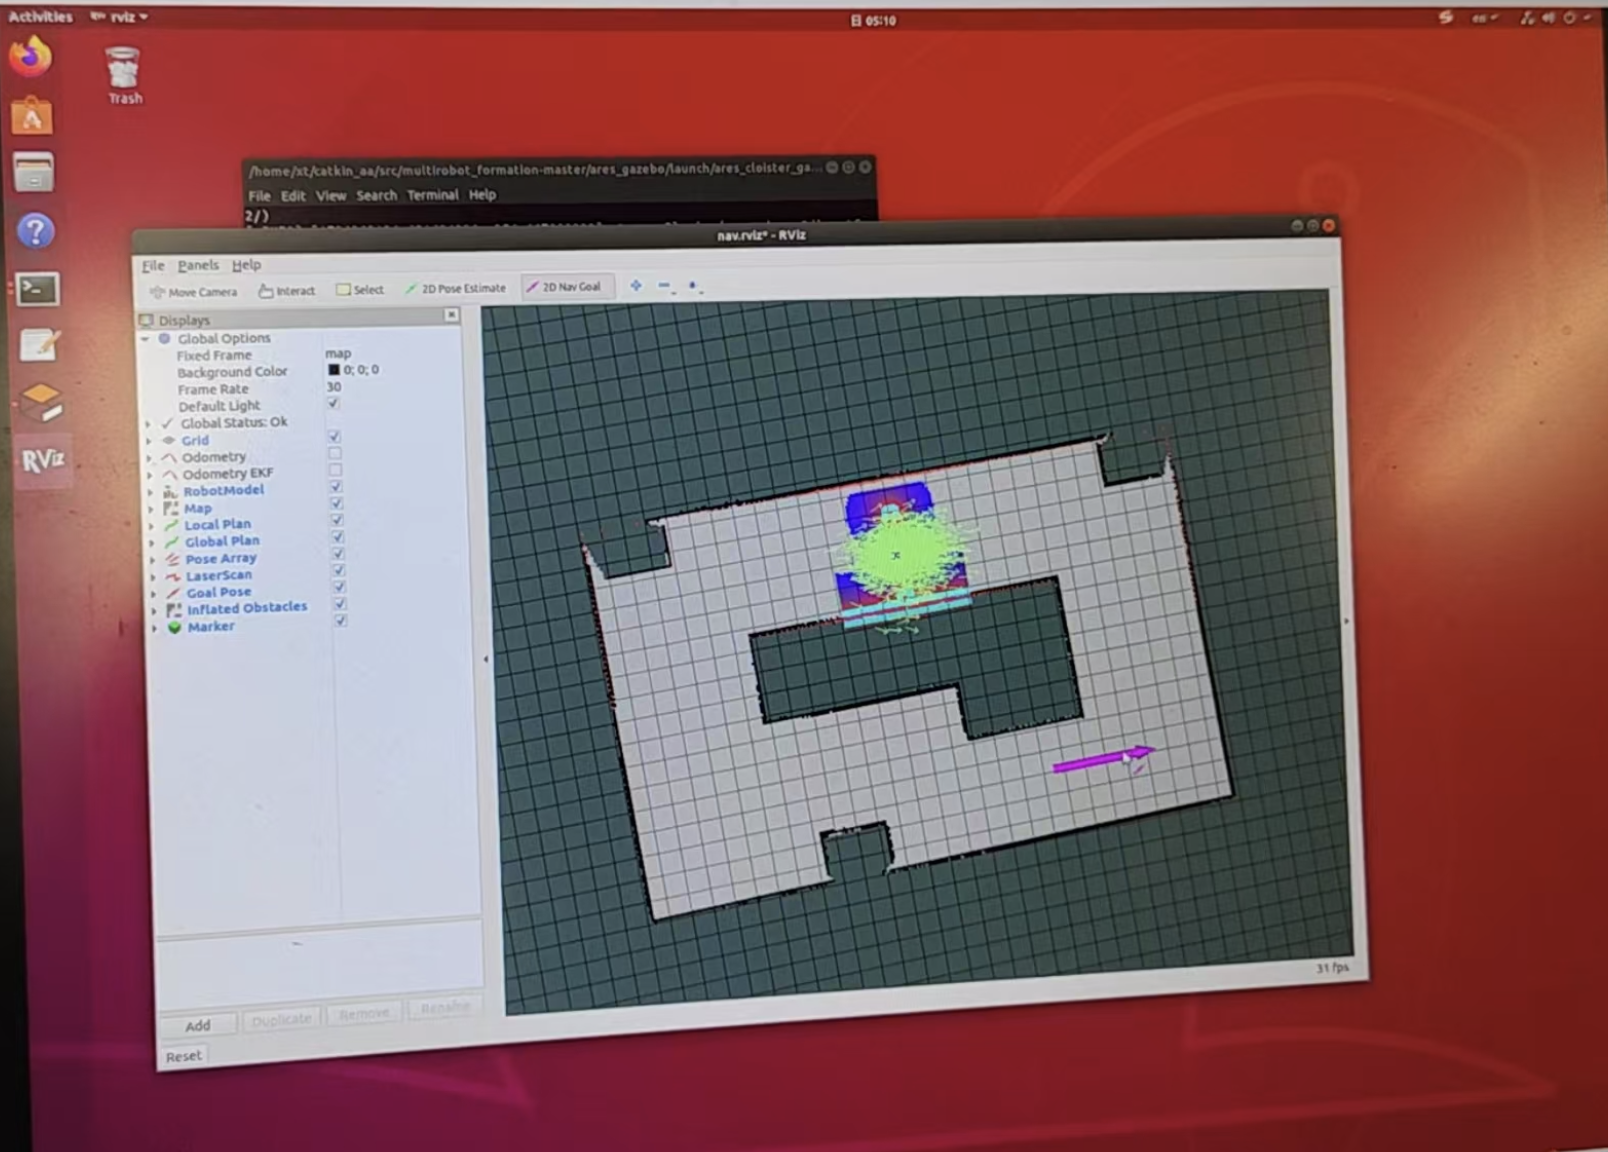
\includegraphics[width=0.8\linewidth]{img/4}
      \caption{机器人导航路径示意图}
\end{figure}
 
\subsection*{总结与展望}
 
综上所述,本实验不仅验证了ROS和Gazebo在无人系统自主导航仿真中的应用效果,还展示了多传感器融合和智能算法的重要性。通过这次实践,我们积累了丰富的开发和调试经验,并认识到未来研究的方向,如引入更多类型的传感器、扩大应用场景范围,以及开发更加智能的路径规划和编队控制算法。
\section{结论与展望}
\subsection*{实验资料参考}
本实验参考了以下资源:
\begin{itemize}
   \item \textbf{古月居多机器人导航教程}:提供了详细的导航算法实现和优化指南。
   \item \textbf{CSDN相关实验说明}:分享了其他研究人员的经验和技巧,帮助解决了遇到的问题。
   \item \textbf{Azure云端实验环境}:利用云计算资源进行大规模仿真测试,提高了实验效率。
\end{itemize}
 
\subsection*{后续改进方向}
 
\subsubsection*{场景复杂性提升}
\paragraph{添加动态障碍物}
为了更真实地模拟现实世界中的情况,未来的研究可以考虑引入动态障碍物。这将增加路径规划算法的挑战性,
并测试其适应性和鲁棒性。例如,在城市环境中模拟行人或车辆的移动,可以更好地评估机器人在复杂交通条件下的表现。
 
\paragraph{更大规模场景分析}
扩大仿真场景的规模,如在一个大型工业园区或城市中心进行多机器人编队测试。这不仅能够检验编队稳定性,
还能探索不同地形对机器人协作的影响。通过这种方式,我们可以发现更多实际应用场景中可能遇到的问题,并提前找到解决方案。
 
\subsubsection*{算法优化}
\paragraph{高效路径规划算法}
采用更高效的路径规划算法,如RRT*(快速随机树)、A*等,以缩短任务完成时间。这些算法能够在保证路径安全的前提下,
尽可能减少行驶距离和能耗。此外,还可以结合机器学习方法,使机器人能够根据历史数据自主优化路径选择策略。
 
\paragraph{改进编队调整策略}
增强编队调整策略,确保队列的一致性和灵活性。例如,引入基于行为的控制方法,
使每个机器人可以根据实时感知信息灵活调整自身位置;或者使用分布式优化算法,让整个编队作为一个整体来响应外部变化。
这样不仅可以提高编队效率,还能增强系统的容错能力。
 
\subsubsection*{硬件验证}
\paragraph{应用于真实机器人平台}
将仿真结果应用于真实的机器人平台,如地面车、无人机等,以验证其在实际环境中的性能。
通过这种方式,可以发现仿真与现实之间的差异,并针对性地改进算法和系统设计。
例如,在户外环境下测试GPS信号干扰问题,或在室内环境中评估传感器精度。
 
\subsubsection*{可视化增强}
\paragraph{轨迹历史记录功能}
添加轨迹历史记录功能,便于复盘分析。该功能可以帮助研究人员回顾机器人的运动轨迹,
分析路径规划的效果,并找出需要改进的地方。例如,通过对比不同算法生成的路径,
直观地展示哪种方法更加优越。
 
\paragraph{优化RViz界面显示}
进一步优化RViz界面显示,使其更加直观易用。例如,增加更多的交互选项,让用户可以直接操作虚拟物体;
或者开发新的插件,支持更多类型的传感器数据展示。这将极大地提升实验的用户体验,
并为教学和演示提供更好的工具。
 
\subsection*{实验扩展与经验总结}
 
\subsubsection*{通过本次实验,我们验证了ROS系统在多机器人导航与编队仿真中的强大功能,
同时对如何利用Gazebo和RViz工具进行了深入探索。这一过程体现了以下几点关键经验:}
 
\paragraph{环境预设的重要性}
仿真场景的设置直接影响了实验的效率和结果。复杂场景中的障碍物配置能够更好地模拟实际情况,
增强实验可信度。例如,在一个包含多种地形特征的城市环境中,机器人需要应对不同的挑战,如狭窄街道、建筑物遮挡等。这种多样化的环境有助于全面评估系统的性能。
 
\paragraph{模块化设计优势}
ROS的模块化使得各功能组件可以单独调试和组合,提高了开发效率。实验中分离导航与编队功能,
分别优化后再联合测试,效果显著。例如,先确保单个机器人能够在复杂环境中稳定导航,
再逐步加入其他机器人,形成编队。这种方法降低了开发难度,并且更容易发现问题所在。
 
\paragraph{实验记录与复盘}
通过详细记录每一步操作和结果变化,可以为后续研究提供清晰的依据,并发现改进点。
例如,通过对导航路径的回溯,发现某些障碍物配置对路径规划算法提出了更高要求。
这提示我们在设计仿真场景时,要充分考虑到各种可能性,从而提高算法的通用性和适应性。
 
\paragraph{硬件与仿真结合的必要性}
虽然本次实验在仿真中取得了良好结果,但仍需在实际硬件环境中进行测试,以验证其鲁棒性与可扩展性。
例如,在户外环境中测试GPS信号强度和稳定性,或在室内环境中评估激光雷达的测量精度。
只有经过这样的双重验证,才能确保我们的研究成果真正具有实用价值。
 
\subsubsection*{总之,本实验不仅达成了既定目标,还为未来的机器人研究提供了宝贵经验和参考方向。}
综上所述,本实验不仅完成了预定的目标,还揭示了ROS系统在多机器人导航与编队仿真方面的巨大潜力。

通过这次实践,我们不仅掌握了关键技术的应用方法,也积累了丰富的开发和调试经验。
更重要的是,我们认识到持续创新和技术进步的重要性,这将为未来的研究奠定坚实的基础。
无论是改善民生福祉还是加强国防建设,多机器人系统都展现出了巨大的潜力和发展前景。

\section{后文}
\subsection{实验分工}
\begin{itemize}
    \item 陈海弘:论文撰写排版
    \item 方唯特:仿真环境实现
    \item 蒋奥周:ROS环境配置
    \item 刘仲晗:资料查找整理
\end{itemize}

\subsection{视频展示}
\href{https://pan.baidu.com/s/1YnxgZXi0YKYByZcN-seqfw?pwd=e5as}{百度网盘链接}
提取码:e5as
%\section{参考文献}
\begin{thebibliography}{00}
    \bibitem{b1} https://www.guyuehome.com/detail?id=1825473662992330753
    \bibitem{b2} https://www.guyuehome.com/detail?id=1825473664502280193
    \bibitem{b3} https://www.guyuehome.com/detail?id=1825473664502280193
    \bibitem{b4} https://www.guyuehome.com/detail?id=1825473548416528385
\end{thebibliography}
\end{document}
